\chapter{\label{appendix:il2-normalisation}}

\begin{figure}
\centering
\begin{minipage}{.65\textwidth}
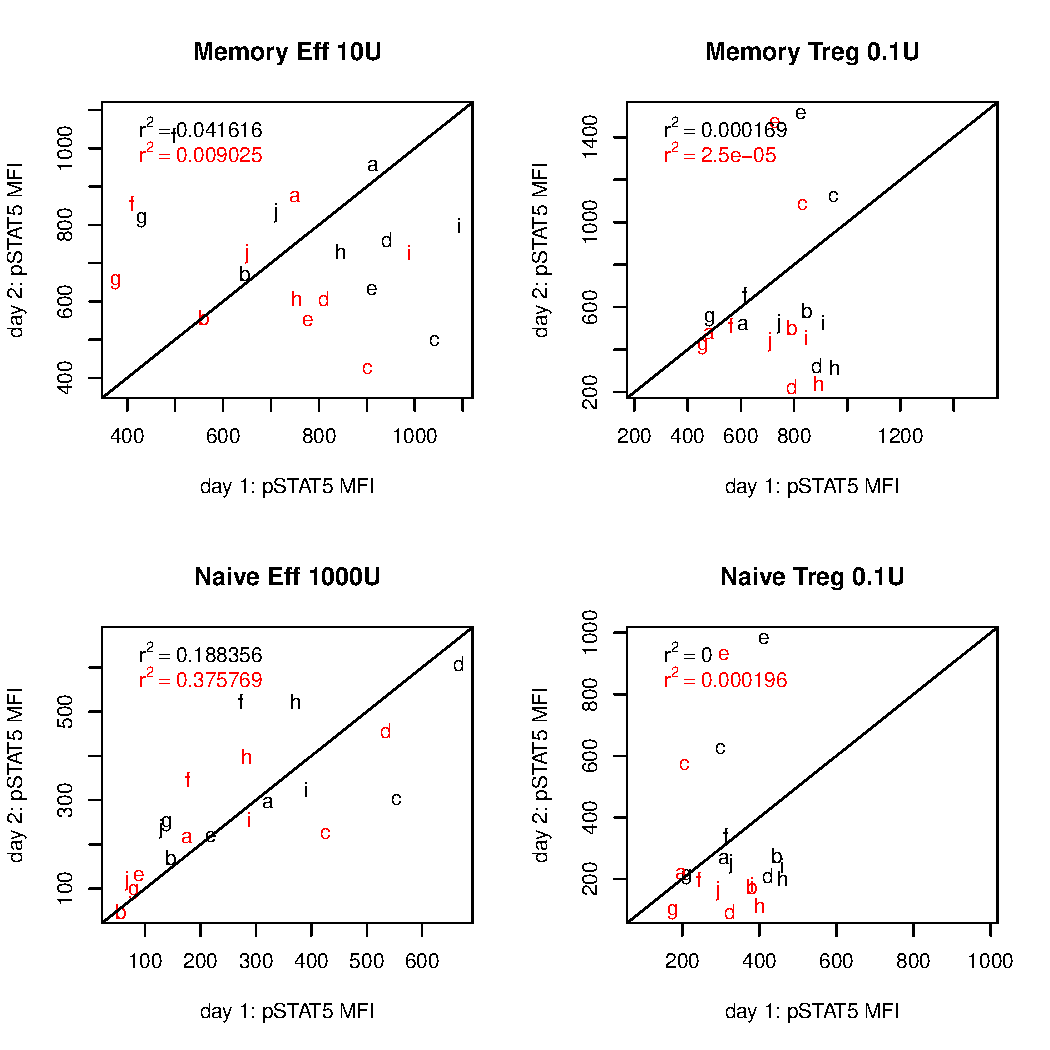
\includegraphics[width=\linewidth]{figures/pstat5-mfi-cellsubsets-repeatability}
\end{minipage}
\begin{minipage}{\textwidth}
\mycaption{figure:pstat5-mfi-cellsubsets-repeatability}
{ Repeatability of pSTAT5 MFI (black) and background corrected pSTAT5 MFI (red). }
{
  Correcting for the MFI in the resting sample does not appear to improve the repeatability significantly but instead just reducing the MFI by the same factor on both days.
  This suggests that the day to day variation in the resting sample MFI does not explain the variation in the stimulated population.
}
\end{minipage}
\end{figure}


\begin{figure}
\centering
%
\begin{minipage}{.65\textwidth}
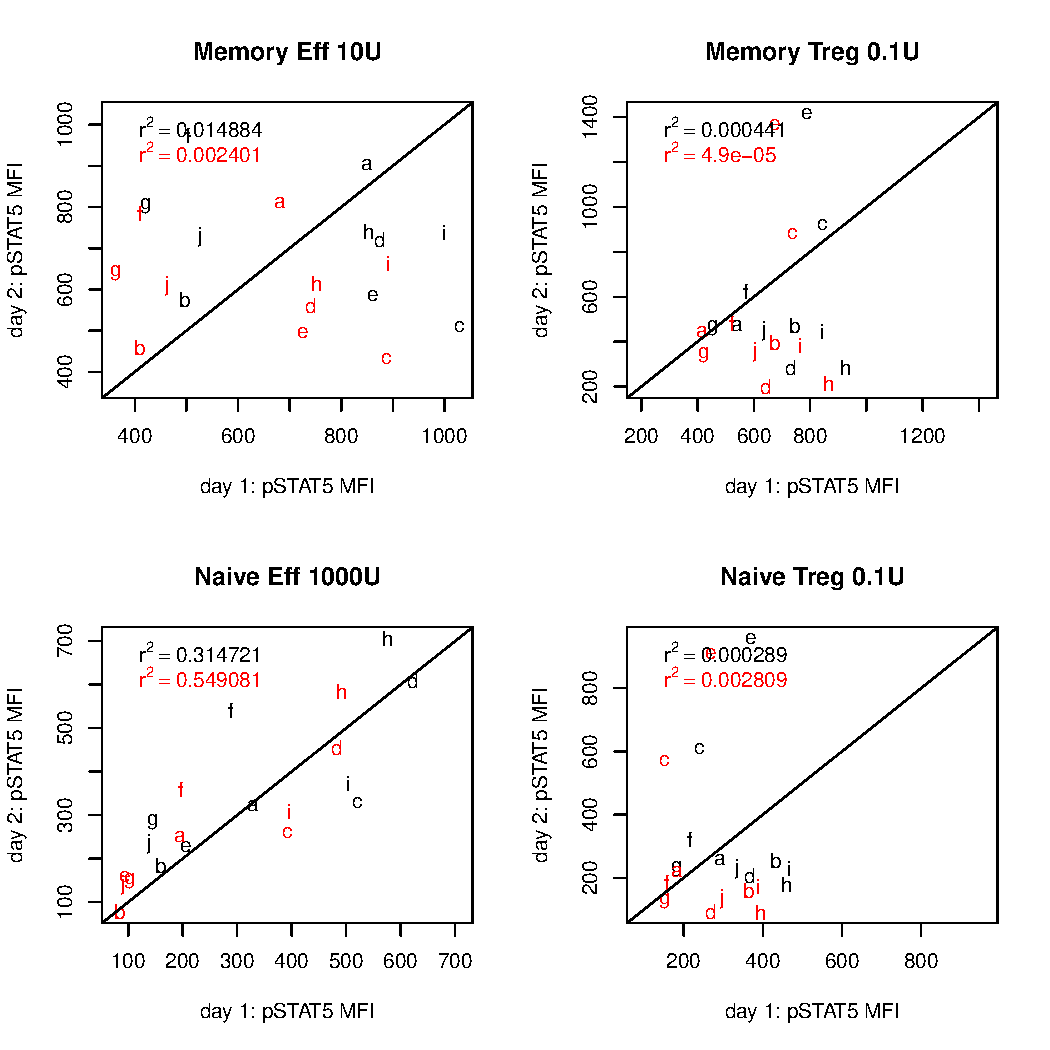
\includegraphics[width=\linewidth]{figures/nn-pstat5-mfi-cellsubsets-repeatability}
\end{minipage}
\begin{minipage}{.3\textwidth}
\mycaption{figure:nn-pstat5-mfi-cellsubsets-repeatability}
{ Repeatability of pSTAT5 MFI in the nearest-neighbour joined (black), nearest-neighbour background subtracted (red). }
{
  %nearest-neighbour joined samples (black)
  %nearest-neighbour joined samples baseline corrected (red)
  %Background subtraction does no substantially improve the repeatability of the pSTAT5 MFI phenotype.
  The stimulation doses are selected as those at which the cell subset responds.
}
\end{minipage}
%
\begin{minipage}{.65\textwidth}
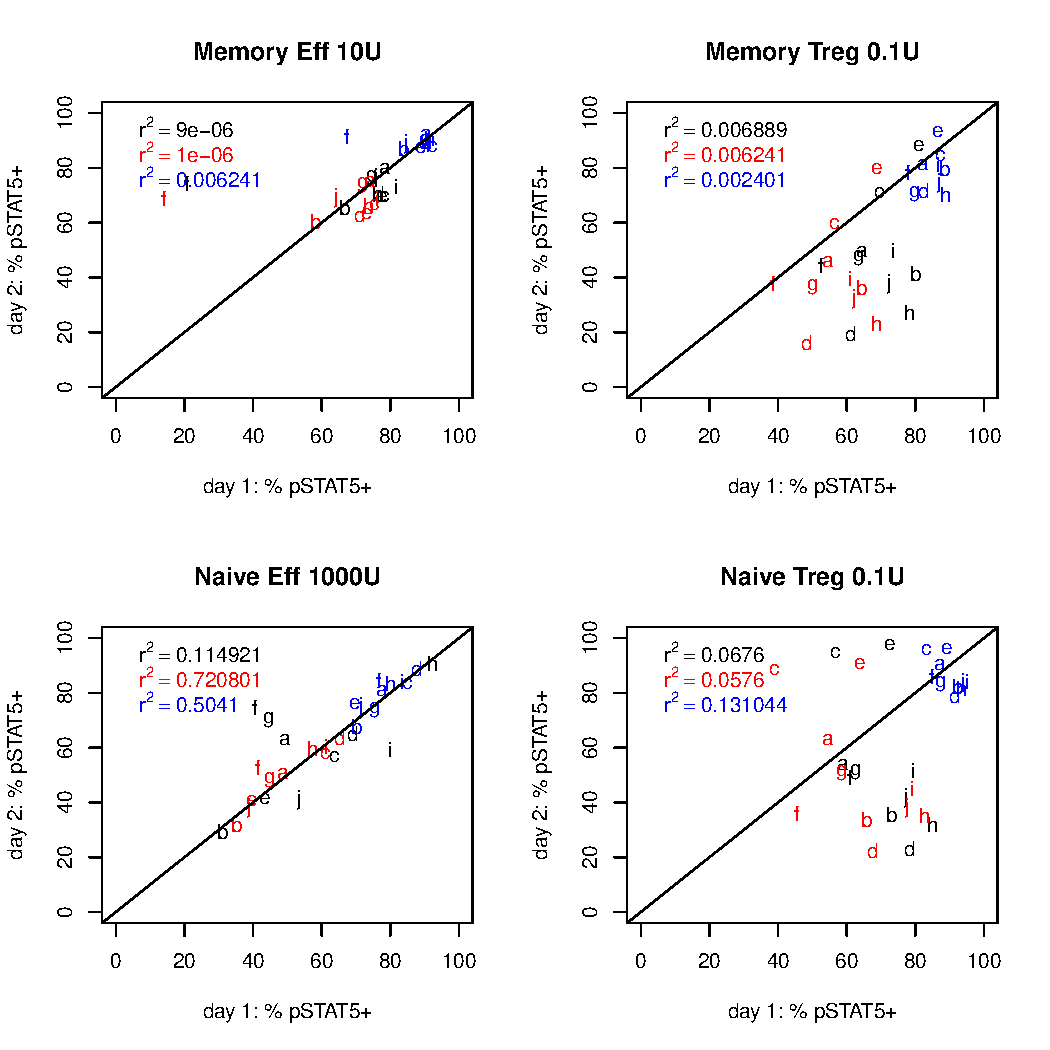
\includegraphics[width=\linewidth]{figures/pstat5-pos-cellsubsets-repeatability}
\end{minipage}
\begin{minipage}{.3\textwidth}
\mycaption{figure:pstat5-pos-cellsubsets-repeatability}
{ Repeatability of percent pSTAT5\positive in the individual samples (black), nearest-neighbour joined (red) and nearest-neighbour joined samples baseline corrected (blue). }
{
  The stimulation doses are selected as those at which the cell subset responds.
}
\end{minipage}
\end{figure}



